\documentclass[12pt]{article}
\usepackage[a4paper,margin=0.75in]{geometry}
\usepackage[utf8]{inputenc}
\usepackage[OT1]{fontenc}
\usepackage[table,usenames,dvipsnames]{xcolor}
\usepackage{array}
\usepackage{varwidth}
\usepackage{tabularx}
\usepackage{amsmath}
\usepackage{hyperref}
\usepackage{enumitem}
\usepackage{graphicx}
\usepackage{tcolorbox}
\usepackage{forest}
\usepackage{parskip}
\renewcommand*\familydefault{\sfdefault}

% from https://gist.github.com/nhtranngoc/88b72d9bfb656a3de227eea38ed80627
\usepackage{listings}
% \usepackage{fontspec}
% \setmonofont{Consolas}

\definecolor{background}{RGB}{39, 40, 34}
\definecolor{string}{RGB}{230, 219, 116}
\definecolor{comment}{RGB}{117, 113, 94}
\definecolor{normal}{RGB}{248, 248, 242}
\definecolor{identifier}{RGB}{166, 226, 46}

\lstset{
  % language=c,                			% choose the language of the code
  numbers=left,                   		% where to put the line-numbers
  stepnumber=1,                   		% the step between two line-numbers.        
  numbersep=5pt,                  		% how far the line-numbers are from the code
  numberstyle=\scriptsize\color{black}\ttfamily,
  backgroundcolor=\color{background},  		% choose the background color. You must add \usepackage{color}
  showspaces=false,               		% show spaces adding particular underscores
  showstringspaces=false,         		% underline spaces within strings
  showtabs=false,                 		% show tabs within strings adding particular underscores
  tabsize=4,                      		% sets default tabsize to 2 spaces
  captionpos=b,                   		% sets the caption-position to bottom
  breaklines=true,                		% sets automatic line breaking
  breakatwhitespace=true,         		% sets if automatic breaks should only happen at whitespace
  title=\lstname,                 		% show the filename of files included with \lstinputlisting;
  basicstyle=\color{normal}\ttfamily\footnotesize,	    	% sets font style for the code
  keywordstyle=\color{magenta}\ttfamily,	% sets color for keywords
  stringstyle=\color{string}\ttfamily,		% sets color for strings
  commentstyle=\color{comment}\ttfamily,	% sets color for comments
  emph={format_string, eff_ana_bf, permute, eff_ana_btr},
  emphstyle=\color{identifier}\ttfamily
}

\newtcolorbox{mybox}[3][]
{
  colframe = #2!25,
  colback  = #2!10,
  coltitle = #2!20!black,  
  title    = {#3},
  #1,
}

\hypersetup{
    colorlinks=true,
    linkcolor=blue,
    filecolor=magenta,      
    urlcolor=cyan,
    pdftitle={Overleaf Example},
    pdfpagemode=FullScreen,
}

\title{\textbf{COL331 Assignment 1}}
\author{Aniruddha Deb \\ \texttt{2020CS10869}}
\date{February 2023}

\begin{document}

\maketitle

\section{Install Linux}

\subsection{MacOS}

The first attempt of the assignment was using QEMU on my Mac. Ubuntu Server 
22.04 was used, and the initial 20GB disk was partitioned into a 1GB boot
and 19GB root partition. The kernel images were kept in boot and everything
else went in the root partition. Installing linux was done by downloading the
kernel tarball (downloads from the git repo were very slow), decompressing it
and following the instructions as mentioned in the assignment. An extra 
parameter, \texttt{CONFIG\_SYSTEM\_REVOCATION\_KEYS}, also had to be set to \texttt{""}
to let the kernel compile. All other parameters were kept as is, and defaults
were used.

The kernel took around 6-7 hours to compile (on a dual core virtualized machine),
and I realized that this approach was infeasible if I was to actually develop
on the kernel.

\subsection{GCP}

After slow compile times on my Mac, I decided to move to Google Cloud Platform.
They offer \$300 worth of free credit, and their compute VM's support ubuntu
server 22.04.1

On an eight core E2-highcpu instance, the kernel compiled in around 35-40
minutes. Installing modules and the kernel itself took another 5-10 minutes.
The only issue was that you couldn't see the grub screen on boot, so the 
installed kernel had to be made the default. This is done by default when you
run the \texttt{make install} command, so nothing had to be changed.

Running \texttt{uname -r} on the VM after bootup shows the kernel as \texttt{6.1.6},
showing that the new kernel was successfully installed (default kernel is 5.15.6)

\begin{mybox}{Goldenrod}{Contingency Management}
Not having access to grub takes away the ability to boot into 5.15 if something
goes wrong, such as if you changed a part of the bootloader code and the kernel
won't boot, and neither can you SSH onto it to edit it. In this case, GCP
provides recovery instructions. The gist of the recovery instructions are that
you need to create a new boot disk, boot the VM using that boot disk, mount the
old boot disk manually and then do recovery, or tweak the grub config on the
old boot disk.
\end{mybox}

\begin{mybox}{Goldenrod}{Ramdisk compression}
The initial image that the bootloader loads into memory (before the filesystem
is initialized) is called a \textbf{ramdisk}. This is make using the kernel
image and the \texttt{mkinitramfs} command, which compresses the image and a
few modules together, which are then loaded into memory.

The ramdisk generated by 6.1.6 compilation with all the default modules takes 
up a lot of space (~500 MB). This can be reduced by not bundling in most of
the modules, but only the dependent ones by changing the \texttt{MODULES}
parameter in \texttt{/etc/initramfs-tools/initramfs.conf} to \texttt{dep} so 
that the compressor guesses which modules to include.
\end{mybox}

\begin{mybox}{ForestGreen}{Kernel Configuration}
Copying and pressing enter for all the options is an inefficient way to
configure the kernel, as most of the modules that it would compile are not used
by the VM (eg filesystems, display drivers, network adapters, device drivers).
You can run \texttt{make menuconfig} to launch a GUI that lets you configure
which parts of the linux kernel to compile. This reduces the size of the kernel
source on disk after build, and also reduces kernel compilation times by 50-60\%.
\end{mybox}

\vspace{1cm}

\begin{figure}[!htbp]
    \centering
    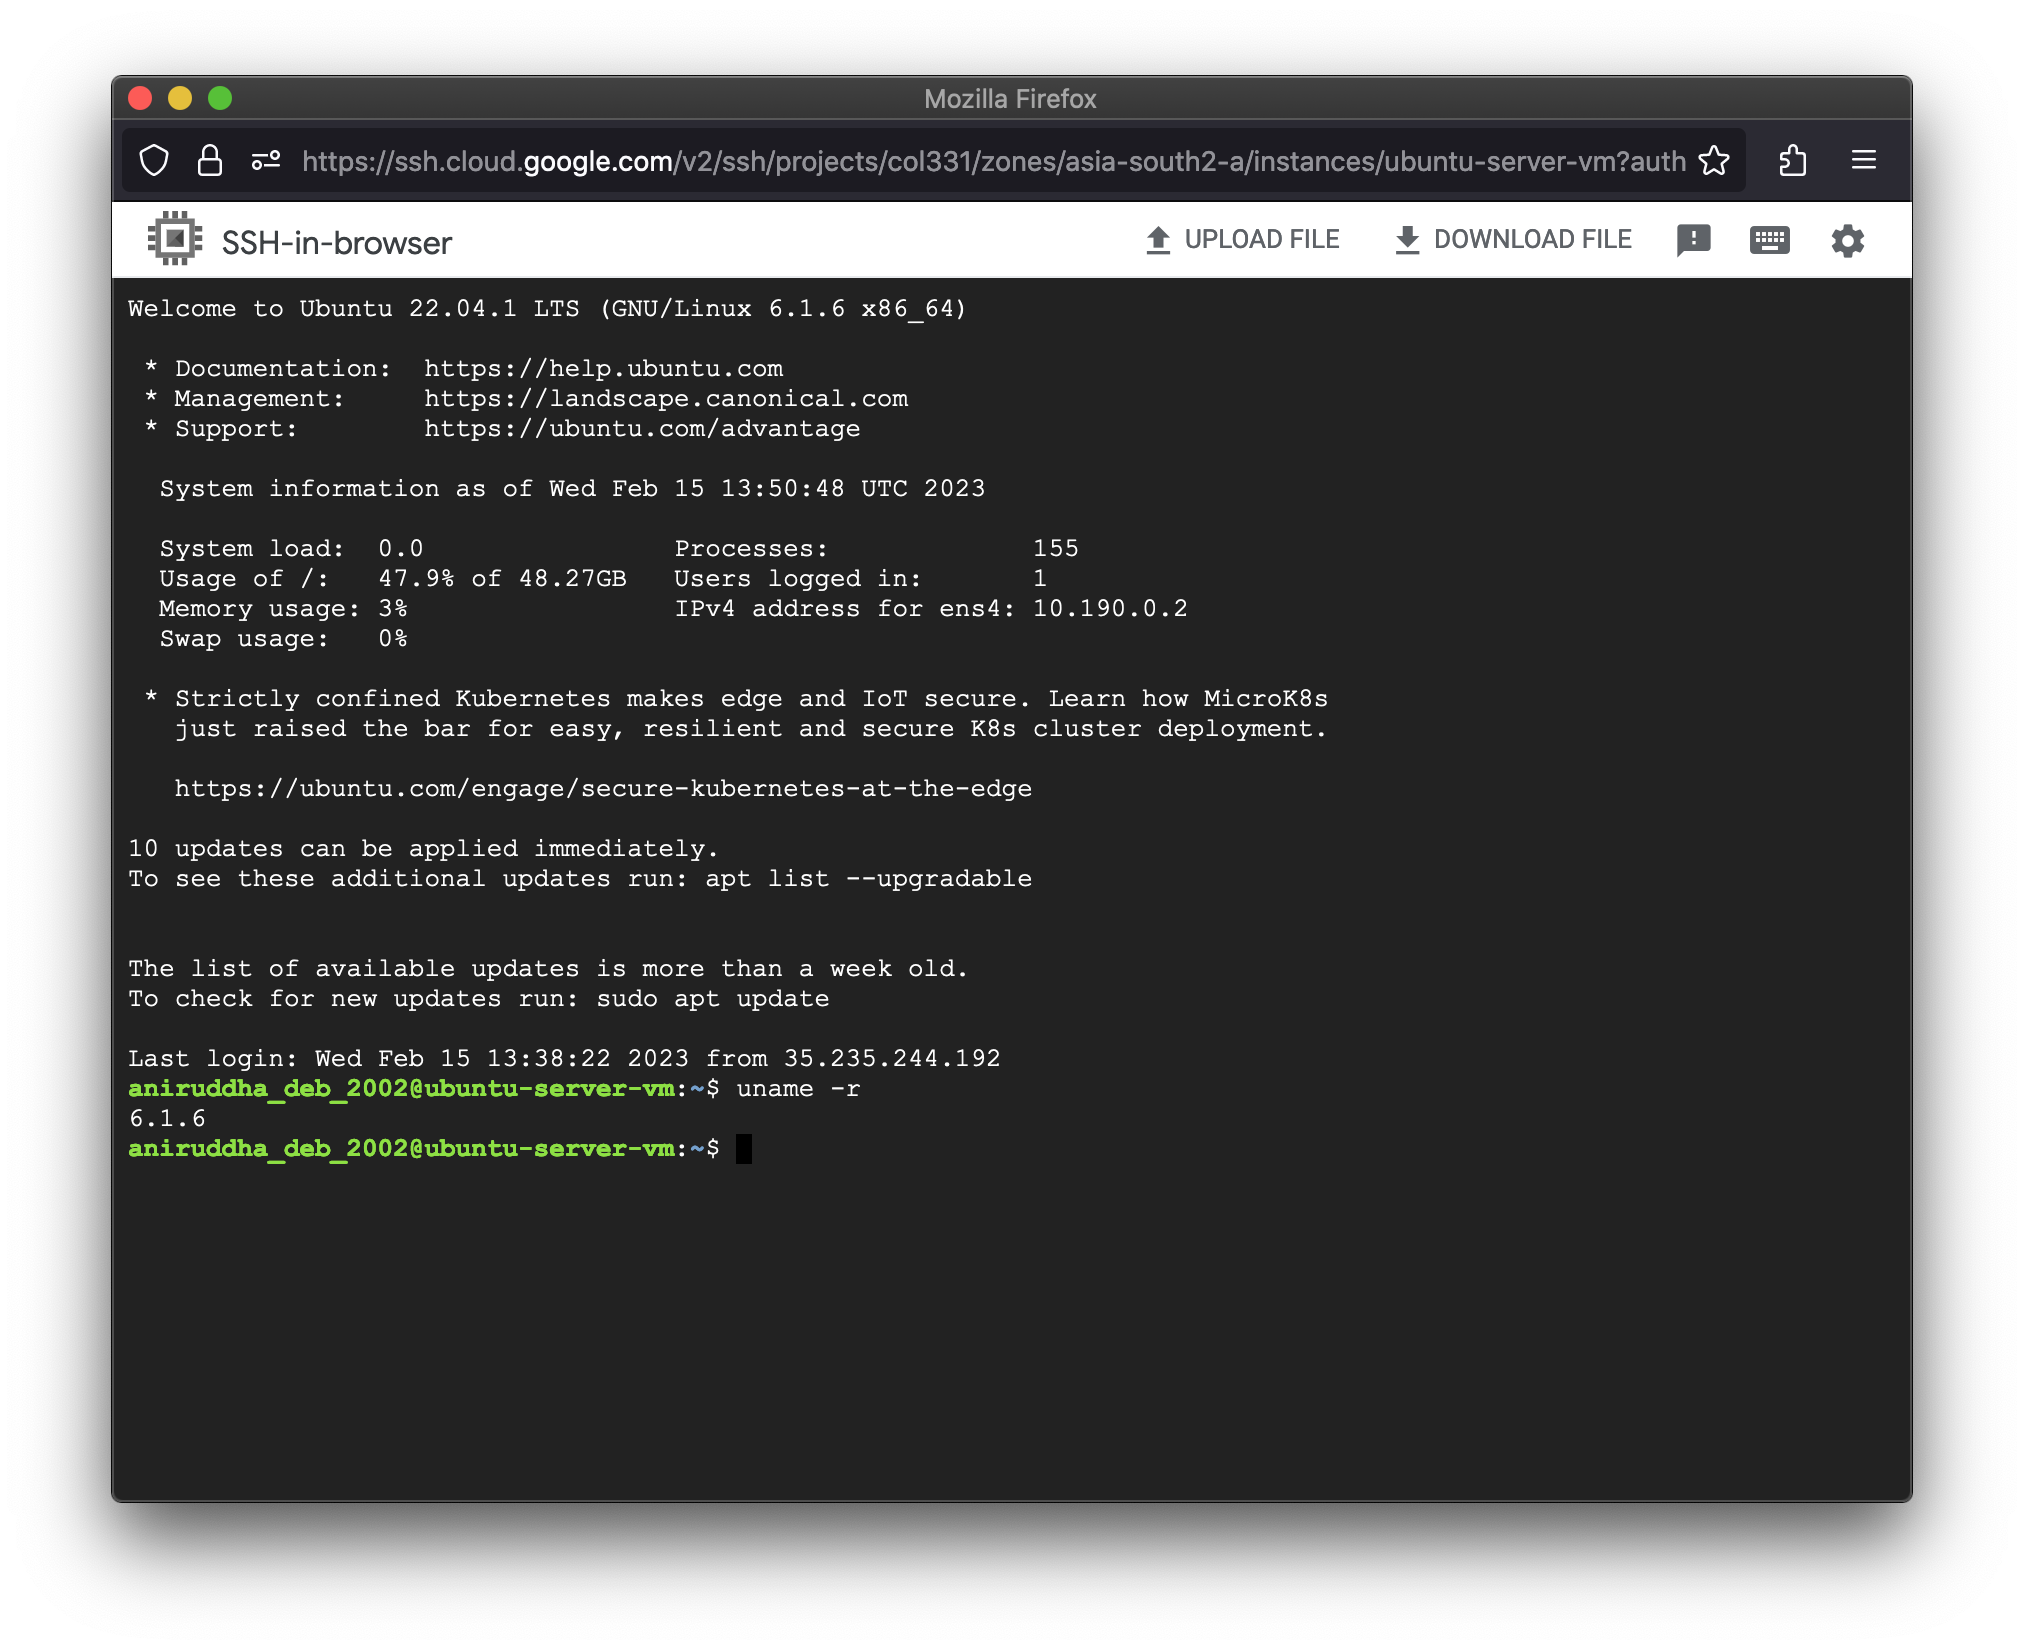
\includegraphics[width=0.8\textwidth]{gcp_vm.png}
    \caption{Google Compute Engine VM (8 cores, 8 GB RAM) on compiled kernel}
\end{figure}

\pagebreak 

\section{System Calls}

% added the data structures in pid.h
% reference: https://brennan.io/2016/11/14/kernel-dev-ep3/
% edited the syscall table to add the syscall
For adding system calls, 
\href{https://www.kernel.org/doc/html/v4.12/process/adding-syscalls.html}
{The kernel.org documentation} and
\href{https://brennan.io/2016/11/14/kernel-dev-ep3/}{Stephen Brennan's Tutorial}
were used. The first edit was to add the structures used to \texttt{include/linux/pid.h},
so that they can be used across the system.

After this, the system call tables were edited to add entries for the three
system calls (note that we call \texttt{register} as \texttt{registr} as the 
former is a reserved C keyword). For symmetry, \texttt{deregistr} is also
similarly named.

In \texttt{syscall\_32.tbl}:
\begin{lstlisting}[language=C]
451	i386	registr		sys_registr
452	i386	fetch		sys_fetch
453	i386	deregistr	sys_deregistr 
\end{lstlisting}

In \texttt{syscall\_64.tbl}:
\begin{lstlisting}[language=C]
548	common	registr		sys_registr
549	common	fetch		sys_fetch
550	common	deregistr	sys_deregistr 
\end{lstlisting}

In \texttt{unistd.h} (\texttt{\_\_NR\_SYSCALLS} was also updated):
\begin{lstlisting}[language=C]
#define __NR_registr 451
__SYSCALL(__NR_registr, sys_registr)
#define __NR_fetch 452
__SYSCALL(__NR_fetch, sys_fetch)
#define __NR_deregistr 453
__SYSCALL(__NR_deregistr, sys_deregistr)
\end{lstlisting}

The syscalls were then linked in \texttt{syscalls.h}
\begin{lstlisting}[language=C]
asmlinkage int sys_registr(pid_t pid);
asmlinkage int sys_fetch(struct pid_ctxt_switch *stats);
asmlinkage int sys_deregistr(pid_t pid);
\end{lstlisting}

Finally, the actual syscalls were implemented in a new file, 
\texttt{kernel/ctx\_switch.c}

\begin{lstlisting}[language=C]
SYSCALL_DEFINE1(registr, pid_t, pid) { ... }
SYSCALL_DEFINE1(fetch, struct pid_ctxt_switch*, pid) { ... }
SYSCALL_DEFINE1(deregistr, pid_t, pid) { ... }
\end{lstlisting}

And this file is added to the Makefile in the \texttt{kernel} directory.
\begin{lstlisting}[language=C]
obj-y += ctx_switch.o
\end{lstlisting}

\subsection{\texttt{registr}}

The \texttt{registr} syscall is implemented using a linked list: after the 
appropriate range checks for the pid, all we do is append a node to the linked
list with the appropriate PID when the system call is called. The new node is
allocated in kernel space, using \texttt{kmalloc}.

\begin{lstlisting}[language=C]
tmp = kmalloc(sizeof(*tmp), GFP_KERNEL);
tmp->pid = pid;

list_add_tail(&tmp->next_prev_list, &pid_ll);
\end{lstlisting}
\texttt{GFP} stands for \textit{Get Free Pages}. More information on kernel
memory allocation was taken from 
\href{https://www.kernel.org/doc/html/v5.18/core-api/memory-allocation.html}{this reference}.

\begin{mybox}{ForestGreen}{Limiting the number of pids}
A possible security vulnerability here is that a user may spuriously add several
billion pid's and use up all the kernel memory. The implementation takes care
of this by setting a limit on the number of pid's that can be kept track of 
(currently 256)
\end{mybox}

\subsection{\texttt{fetch}}

The \texttt{fetch} syscall iterates over all the members of the linked list
using the \texttt{list\_for\_each\_entry} macro, obtaining the task struct
corresponding to the given pid. If the struct exists, it accumulates the
\texttt{nvcsw} and \texttt{nivcsw} values to a local variable. It then copies
the values in the local variable to user memory using \texttt{copy\_to\_user}. 

\begin{lstlisting}[language=C]
struct pid_ctxt_switch pid_stats = {.nvctxt = 0, .ninvctxt = 0};
struct pid_node *n;

list_for_each_entry(n, &pid_ll, next_prev_list) {
    // if task exists, add stats to pid_stats
}

if (copy_to_user(pid, &pid_stats, sizeof(pid_stats))) return -EINVAL;
\end{lstlisting}

\begin{mybox}{Goldenrod}{Reallocated pid's?}
If a pid registered with this syscall is reallocated, then we may obtain spurious
numbers. I couldn't find a way to find out if a pid has been reallocated, so
this bug exists.
\end{mybox}

\subsection{\texttt{deregistr}}

The \texttt{deregistr} syscall looks for the given pid in the list. If the pid
is found, it deletes it and decrements the number of pids registered by one.

\begin{lstlisting}[language=C]
struct pid_node *n;
char found = 0;

list_for_each_entry(n, &pid_ll, next_prev_list) {
    // if pid matches, found = 1 and break
}

if (found) {
    // remove n from pid_ll, free memory for the node 
    // and decrement n_pids by 1
}
\end{lstlisting}

\begin{mybox}{red}{Synchronization?}
When SMP was first introduced, the entire kernel was locked using a Big Kernel 
Lock (BKL). Now, synchronization in the kernel is more fine-grained. I couldn't
find an authoritative resource to check if system calls are multithreaded or 
not, and if race conditions can originate if, say two users call the system
call (one calls fetch and one calls register). Since performance is of most
importance, I refrained from locking the list here.
\end{mybox}

\subsection{Testing}

A test was written to test the three syscalls and placed in the 
\texttt{tools/testing/selftests} directory. This test takes in pids as command
line arguments, adds all the pids passed via the \texttt{registr} syscall, 
fetches the total voluntary and involuntary context switches and finally
deregisters all the registered pids.


\begin{lstlisting}[language=C]
int *pids = (int*)malloc(sizeof(int)*(argc-1));
char *p;
for (int i=1; i<argc; i++) {
    pids[i-1] = (int)strtol(argv[i], &p, 10);
    if (syscall(548, pids[i-1]) != 0) {
        // error
        printf("ERROR: could not register process %d, syscall returned %d\n", pids[i-1], errno);
    }
}

printf("Registered all processes\n");

// fetch the changes
struct pid_ctxt_switch *ctx_switch = (struct pid_ctxt_switch*)malloc(sizeof(struct pid_ctxt_switch));
if (syscall(549, ctx_switch) != 0) {
    printf("ERROR: could not fetch context switches, syscall returned %d\n", errno);
}

// print the switches
printf("Voluntary changes: %lu\n", ctx_switch->nvctxt);
printf("Involuntary changes: %lu\n", ctx_switch->ninvctxt);

// deregister processes
for (int i=0; i<argc-1; i++) {
    if (syscall(550, pids[i]) != 0) {
        printf("ERROR: could not deregister pid %d, syscall returned %d\n", pids[i], errno);
    }
}

printf("Deregistered all processes\n");
\end{lstlisting}

\pagebreak

\section{Kernel Module}

The kernel module was separately implemented in the \texttt{sig\_mod.c} file,
outside the kernel. The module uses a linked list to store (pid,signal) pairs
whose size is limited to 256 pairs (to avoid the overflow described previously).
Every second, the module iterates over all the items in the list, and sends the
appropriate signal to the corresponding pid. 

On being loaded, the module creates the procfile, initializes the pid list 
mutex and sets the timer to execute after one second. On being removed, the 
module cleans up all nodes in the list, deletes the timer (synchronously, which
waits if a timer event is running to complete) and then destroys the list mutex

\subsection{Proc file I/O}
Newer iterations of the linux kernel feature a newer proc filesystem API, which
is not particularly well documented. I used 
\href{https://devarea.com/linux-kernel-development-creating-a-proc-file-and-interfacing-with-user-space/}
{this reference} for writing the write and read handlers, and seeing how to 
register/deregister proc files with the kernel.

\begin{lstlisting}[language=C]
static struct proc_dir_entry *sig_target;

static ssize_t sig_tgt_read(struct file *file, char __user *ubuf, size_t count, loff_t *ppos) {
    char buf[BUFSIZE];
    int len=0;
    if(*ppos > 0 || count < BUFSIZE)
    	return 0;
    // write to buffer here using sprintf
    if(copy_to_user(ubuf,buf,len))
    	return -EFAULT;
    *ppos = len;
    return len;
}

static ssize_t sig_tgt_write(struct file *file, const char __user *ubuf, size_t count, loff_t *ppos) {
    int num,c;
    char buf[BUFSIZE];
    if(*ppos > 0 || count > BUFSIZE)
    	return -EFAULT;
    if(copy_from_user(buf, ubuf, count))
    	return -EFAULT;
    // read from buf here using sscanf
    // create a node and add it to the list using the values read
    c = strlen(buf);
    *ppos = c;
    return c;
}

static const struct proc_ops sig_target_ops = {
    .proc_write = sig_tgt_write,
    .proc_read = sig_tgt_read
};

// register sig_target = proc_create(PROCFILE_NAME, 00622, NULL, &sig_target_ops);
\end{lstlisting}

This is safe from buffer overflows.

\begin{mybox}{ForestGreen}{Procfile permissions}
The permissions for the procfile are set to \textbf{0622}. This gives \textbf{only root}
the ability to read the registered signals, and not users. This prevents one
user from seeing the signals and processes registered by another user, making
this module secure.
\end{mybox}

\subsection{Timer}

A 1 second timer is used to periodically send signals to the registered processes.
The implementation details were taken from \textit{Linux Kernel Development, 3rd ed.}
by Robert Love (chapter 11). The timer takes a function to callback while being
defined, and then is set to be called at a certain duration in the future. 

\begin{lstlisting}[language=C]
void send_signals(struct timer_list* timer) {

    // lock mutex
    // for each entry, send a signal
    //     If the task_struct for the entry is not found, delete it
    // unlock mutex

    // so that the timer is again called after 1s
    mod_timer(timer, jiffies+DELAY);
}

DEFINE_TIMER(timer, send_signals);

\end{lstlisting}

The signals themselves are sent using the \texttt{send\_sig\_info} function,
which takes in a \texttt{kernel\_siginfo} struct whose field \texttt{si\_signo}
is set to the required signal number. 

The timer is registered on startup using \texttt{add\_timer} and deregistered 
on shutdown using \\ \texttt{del\_timer\_sync}, which, as previously described,
waits for timer callbacks (if any) to terminate.

\subsection{Synchronization}

All accessess to the pid list are thread-safe and locked via a mutex: this is
to allow multiple users to safely add signal requests without leading to race
conditions. According to \href{https://unix.stackexchange.com/questions/186355/few-questions-about-system-calls-and-kernel-modules-kernel-services-in-parallel}
{this source}, module calls may be called in parallel on a multi-user, multi-cpu 
system, and hence this safety is neccessary. The mutex is implemented using
the methods in \texttt{include/linux/mutex.h}

\begin{lstlisting}[language=C]
DEFINE_MUTEX(mutex);

mutex_init(&mutex);

mutex_lock(&mutex);
// critical code accessing pid linked list
mutex_unlock(&mutex);

mutex_destroy(&mutex);
\end{lstlisting}

\begin{mybox}{red}{DoS attack on file}
By sending in a large number of pids, one expects that the system goes into 
starvation while adding the pids to the file and not giving up the lock, thereby
preventing the timer callback from sending signals. This is prevented to a degree
by limiting the number of such requests. However, this check is done in a
synchronous fashion, hence it is possible that the system does get starved. I
would need a lock-free algorithm that can check the length of the list as well
as add (not remove) to the list to prevent this from happening.
\end{mybox}

\section{Submission Details}

The diff file was generated after cleaning the build directory using \texttt{make mrproper},
and running \texttt{git diff --no-index <original> <new> --output ctxtswitch.patch}.
This patch is compatible with the kernel and can be applied, with the benefit
of being much smaller than the patch generated by the command mentioned. Git 
diff respects the .gitignore files in the directories thereby making a much
smaller patch file.

The directory structure is as follows:

{\footnotesize
\begin{forest}
  for tree={
    font=\ttfamily,
    grow'=0,
    child anchor=west,
    parent anchor=south,
    anchor=west,
    calign=first,
    edge path={
      \noexpand\path [draw, \forestoption{edge}]
      (!u.south west) +(5pt,0) |- node[fill,inner sep=1.25pt] {} (.child anchor)\forestoption{edge label};
    },
    before typesetting nodes={
      if n=1
        {insert before={[,phantom]}}
        {}
    },
    fit=tight,
    before computing xy={l=15pt},
  }
[assignment1\_hard\_2020CS10869
  [ctxttrack.patch]
  [report.pdf]
  [sig\_mod
    [Makefile]
    [sig\_mod.c]
  ]
]
\end{forest}
}

The kernel module can be made using the \texttt{make} command, and loaded/removed 
using \texttt{sudo insmod} and \texttt{sudo rmmod}.

\end{document}
